\documentclass[tikz,border=8pt]{standalone}
\usepackage{amsmath,amssymb}
\usepackage{xeCJK}
\setCJKmainfont{Noto Serif CJK SC}
\usetikzlibrary{arrows.meta}
\begin{document}
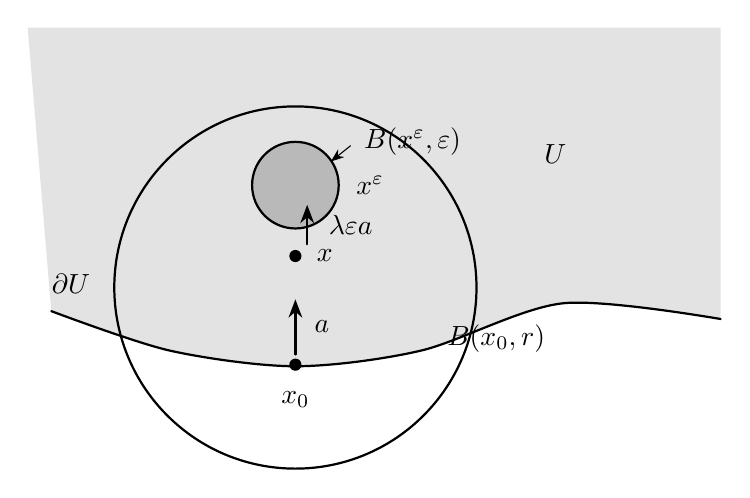
\begin{tikzpicture}[x=1cm,y=1cm,>=Stealth,line cap=round,line join=round]
% ---------- boundary and domain U ----------
\def\boundary{(0.3,3.4) (1.8,2.9) (3.4,2.7) (5.0,2.9) (6.8,3.5) (8.8,3.3)}
\fill[gray!22] (0.0,7.0) -- (0.3,3.4)
  -- plot[smooth] coordinates {\boundary}
  -- (8.8,7.0) -- cycle;
\draw[thick] plot[smooth] coordinates {\boundary};
\node at (0.55,3.75) {$\partial U$};
\node at (6.7,5.4) {$U$};
% ---------- large ball ----------
\draw[thick] (3.4,3.7) circle (2.3);
\node at (5.95,3.05) {$B(x_0,r)$};
% ---------- points ----------
\fill (3.4,2.72) circle (2.2pt);
\node[below] at (3.4,2.5) {$x_0$};
\fill (3.4,4.1) circle (2.2pt);
\node[right] at (3.55,4.1) {$x$};
\fill (3.4,5.0) circle (2.2pt);
\node[right] at (4.05,5.0) {$x^\varepsilon$};
% ---------- small ball ----------
\fill[gray!55] (3.4,5.0) circle (0.55);
\draw[thick] (3.4,5.0) circle (0.55);
\node[right] at (4.15,5.55) {$B(x^\varepsilon,\varepsilon)$};
\draw[->] (4.1,5.5) -- (3.85,5.3);
% ---------- translation ----------
\draw[->,thick] (3.55,4.25) -- (3.55,4.75);
\node[right] at (3.7,4.5) {$\lambda\varepsilon a$};
% ---------- inward normal ----------
\draw[->,thick] (3.4,2.85) -- (3.4,3.55);
\node[right] at (3.52,3.2) {$a$};
\end{tikzpicture}
\end{document}
